\documentclass[conference]{IEEEtran}
\IEEEoverridecommandlockouts
% The preceding line is only needed to identify funding in the first footnote. If that is unneeded, please comment it out.
\usepackage{cite}
\usepackage{amsmath,amssymb,amsfonts}
\usepackage{algorithmic}
\usepackage{graphicx}
\usepackage{textcomp}
\usepackage{xcolor}
\def\BibTeX{{\rm B\kern-.05em{\sc i\kern-.025em b}\kern-.08em
    T\kern-.1667em\lower.7ex\hbox{E}\kern-.125emX}}
    
    
%% my packages %%
\usepackage{hyperref}
\usepackage{tabularx}
\usepackage{pagecolor}
%%%%%%%%%%%

\begin{document}

\pagecolor{white!30}

\title{ECS637U/ECS757P - Digital Media and Social Networks Group Project Deliverable 2}

\author{
\IEEEauthorblockN{Domantas Miliauskas}
\IEEEauthorblockA{\href{mailto:d.miliauskas@se16.qmul.ac.uk}{d.miliauskas@se16.qmul.ac.uk} \\
Introduction, extension work, \\
tabulating results, graph drawing,\\
report writing \\
25\%
}

\and

\IEEEauthorblockN{Gurpal Jabble}
\IEEEauthorblockA{\href{mailto:g.jabble@se16.qmul.ac.uk}{g.jabble@se16.qmul.ac.uk} \\
Problem formulation, algorithm implementation, \\
performing analyses, tabulating results, \\
graph drawing, report writing \\
25\%
}

\and

\IEEEauthorblockN{Harvey Randall}
\IEEEauthorblockA{\href{mailto:h.randall@se16.qmul.ac.uk}{h.randall@se16.qmul.ac.uk} \\
Algorithm implementation, performing analyses, \\
extension work, tabulating results, graph drawing, \\
report writing, \LaTeX writeup \\
25\%
}

\and

\IEEEauthorblockN{Mehmet Keven}
\IEEEauthorblockA{\href{mailto:m.e.keven@se17.qmul.ac.uk}{m.e.keven@se17.qmul.ac.uk} \\
Related work, extension work, \\
report writing \\ 
25\%
}}

\maketitle
\thispagestyle{plain}
\pagestyle{plain}

\begin{abstract}
Abstract?
\end{abstract}

\begin{IEEEkeywords}
\textbf{Modularity}: a measure of the extent to which nodes of the same type are connected to nodes of the same type \\
\textbf{Edge betweenness}: the number of shortest paths between pairs of nodes that run along an edge \cite{b1}
\end{IEEEkeywords}

\section{Introduction}
	{
		The aim of this report is to gain further insight into three Glastonbury festival twitter datasets that consist of tweets collected through different stream collection techniques; Baseline (BL), Adaptive (AD) and Extra (EX). We aim to implement a community detection algorithm on each dataset to detect topic clusters, which will be analysed based on sentiment using Naive Bayes classification methods to determine whether a given cluster contains ‘Good’, ‘Neutral’ or ‘Bad’ tweets.
	\par}

\section{Background}
	\subsection{Sentiment Analysis}
		{
			There has been a growing interest in mining opinions and sentiment through Twitter, as nowadays everything is shared on this social platform with over 250 million tweets being made each day (Twitter, 2012). Many papers are available on the topic of performing sentiment analysis on tweets with the use of machine learning techniques such as the Naïve Bayes classifier, whether it be to see the overall opinion on a social event or to predict the financial market.\\
			
			One paper describes a system for real-time analysis of public sentiment towards presidential candidates in the 2012 US election as expressed on Twitter. They have effectively gathered over 36 million tweets about the election. With this data, they attempt to explore whether Twitter provides insights into the unfolding of the campaigns and indications of shifts in public opinion.\\

			To obtain a labelled train dataset, they used a crowdsourcing approach and used Amazon Mechanical Turk (AMT) to get a varied population of around 800 annotators. They designed an interface that allowed annotators to participate anonymously. They were shown a series of tweets and asked to annotate the tweets' sentiment. As a result, they had 17000 tweets for training.\\
			
			With new tweets coming in, they pre-process them with Christopher Potts’ basic Twitter tokenizer. A Naïve Bayes model on unigram features is used for the classification. The features are calculated from tokenization of the tweets that attempt to preserve punctuation that may signify sentiment as well as twitter specific phenomena. Based on the data collected, their classifier performs at 59\% accuracy on the four-category classification of negative, positive, neutral, or unsure.\\

			In conclusion, one finding is that their infrastructure and sentiment model evaluates public sentiment changes in response to emerging political events and news as they unfold. For instance, during the Republican Primary debate on Jan 19, 2012 in Charleston, NC, Newt Gingrich, a republican candidate, was asked about his ex-wife. His negative sentiment tripled in just two minutes.
		\par}
	
	\subsection{Community Detection}
		{
			Community detection is the process of finding groups of nodes within networks that are highly connected to one another and few connections to nodes outside of this group. When we look at small networks it can be quite easy to detect small communities but when networks become much larger it becomes difficult to identify communities. Identifying communities is worthwhile though as it enables us to find related nodes and can reveal the nature of social interaction within a network. \\
			
			Community detection can be divided into two separate areas: 
				\begin{enumerate}
					\item Hierarchical community detection
					\item Overlapping community detection. 
				\end{enumerate}
			The former involves dividing the network in such a way that nodes can only exist within one community or another but never more than one, whereas the latter allows nodes to exist within multiple communities. We will focus on hierarchical community detection which can again be divided into separate areas: 
				\begin{enumerate}
					\item Divisive detection methods
					\item Agglomerative detection methods
				\end{enumerate}
			Divisive methods can be considered top down approaches to community detection as they begin with the complete network and iteratively remove edges, dividing nodes into separate, more densely connected groups. Agglomerative methods can be considered bottom up approaches to community detection as they initially consider each node as a single community and merge communities until every node belongs to the same community.
			
			One method of edge removal is to remove bridges and local bridges between nodes to produce these new groups of nodes, this can be problematic though as sometimes there may be no bridges or local bridges in the network to remove. Another method is to remove edges using the notion of edge betweenness to find edges that are least central to communities \cite{gnewman}. This is calculated by finding the number of shortest paths between nodes that use this edge. The edge with the highest edge betweenness value is then removed to separate the nodes into separate groups. This approach still allows us to find edges for removal even if bridges do not exist in the network and therefore allows us to still find communities. \\
			This approach runs with time complexity $O(m^{2}n)$ where $m$ is the number of edges in the network and $n$ is the number of nodes. This is not a problem for networks with small $n$ however as networks become larger the time it takes to complete increases rapidly, particularly when trying to find communities in social networks which can have very large $n$ and $m$ values such as the dataset we are working with. \\
			
			Agglomerative methods are performed in the opposite way to divisive methods, taking a bottom-up approach as opposed to a top-down approach. Each node begins as its own cluster and clusters are merged successively until all clusters have been merged into one cluster. One method of doing this is by measuring the Euclidean distance between clusters and merging the closest clusters until one cluster is formed. Euclidean distance is just one example of a distance metric that might be used, another commonly used metric is metric is modularity. Modularity is a measure used in networks to describe the strength of a community division, a high modularity value indicates a set of nodes is densely connected whereas a low modularity value indicates nodes are sparsely connected. Fast agglomerative algorithms can be implemented using greedy optimisation of modularity to efficiently find communities in large networks \cite{cnewman} \cite{louvain} that run with better time complexity than the divisive algorithm described above. These algorithms work by merging clusters which provide the best increase in modularity at each iteration.\\
			These algorithms can be graphically represented by a dendrogram. These visualisations are typically displayed bottom to top, ie at the bottom is each individual community (each node) and as you travel upwards branches show which communities have been merged. 
		\par}
	
	\subsection{\textbf{EXTENSION:} Page Rank and its application to network analysis}
		{
			PageRank is an algorithm used to rank web pages in Google search engine results. It was developed by the founders of Google - Larry Page and Sergey Brin, and its functional prototype was released in 1998. The goal of PageRank is to get a measure of how popular webpages are based on other pages that are linked to them. Since not all links share the same value, the importance of a web page is calculated by the number, as well as the quality of links pointing to that page. PageRank is a recursively defined measure as a page becomes important if important pages link to it. With that said, the underlying assumption is that more important websites are likely to receive more links from other websites.\\
			
			One way to think about PageRank is to imagine a random surfer on the web, following links from page to page. The page rank of any page is roughly the probability that the random surfer will land on a particular page. Since more links go to the important pages, the surfer is more likely to end up there. Google’s random surfer is an example of a Markov process, in which a system moves from state to state, based on probability information that shows the likelihood of moving from each state to every other possible state.\\
			
			When calculating PageRank, the distribution is evenly divided among all webpages at the beginning of the computational process. In a network with n nodes (nodes being webpages), we assign all nodes the same initial PageRank of 1/n. Then, we choose a number of steps k and perform a sequence of k updates to the PageRank values:
			\begin{itemize}
				\item Each page divides its current PageRank equally across its out-going links and passes these equal shares to the pages it points to. Also, if a page has no out-going links, it passes all its current PageRank to itself. Each page updates its new PageRank to be the sum of the shares it receives.
			\end{itemize}
		
		The PageRank computations require several iterations through the collection of webpages to adjust approximate PageRank values to more closely reflect the theoretical true value. This is when we get to the convergence case, where the PageRank values stop changing.
		\par}


\section{Dataset}
	{
		We will be using a dataset of tweets collected during the 2013 Glastonbury Music Festival using a STRIM \cite{strim} framework to collect the tweets and detect sub-event occurrence in real time. This dataset is comprised of three streams: \begin{itemize}
			\item \textbf{Baseline}: the stream of tweets collected from the static user-specified keywords
			\item \textbf{Adaptive}: the stream of tweets collected using the adaptive crawler to dynamically update the keywords
			\item \textbf{Extra}: the stream of tweets collected only by the adaptive crawler ie the difference between the adaptive and baseline streams
		\end{itemize}
		In particular we will be analysing the hashtag co-occurrence network of each of these streams to identify hashtags which are used in combination with one another. Each node of our graphs will represent a hashtag and edges will represent these hashtags being used in the same tweet, the weight of each edge will be determined by the frequency the hashtags are used together: the larger the edge weighting the more frequently they co-occur. Some preprocessing of the data was required to create a co-occurrence list that could be used to create a co-occurrence network. This was done by first loading the SQL files for each stream and iterating over their contents, the hashtags were extracted using a simple SQL query \texttt{SELECT 'hashtags' FROM <table>;} where \texttt{<table>} is the name of the stream. The returned string was split by space and sorted alphabetically, if the resulting list contained more than one element then the results were stored in a dictionary used to count co-occurrence before finally being written to CSV in a format that can be parsed by Gephi as well as networkx. \\
		
		Initial analysis of the network shows that the graph consists mostly of low degree nodes with a rapid decrease in the frequency of nodes with specific frequency as node degree increases demonstrating that our networks display a power law distribution. The graph below shows the frequency of node by node degree shown on a log-log graph. 
	\par}
	\begin{figure}[htbp]
		\centerline{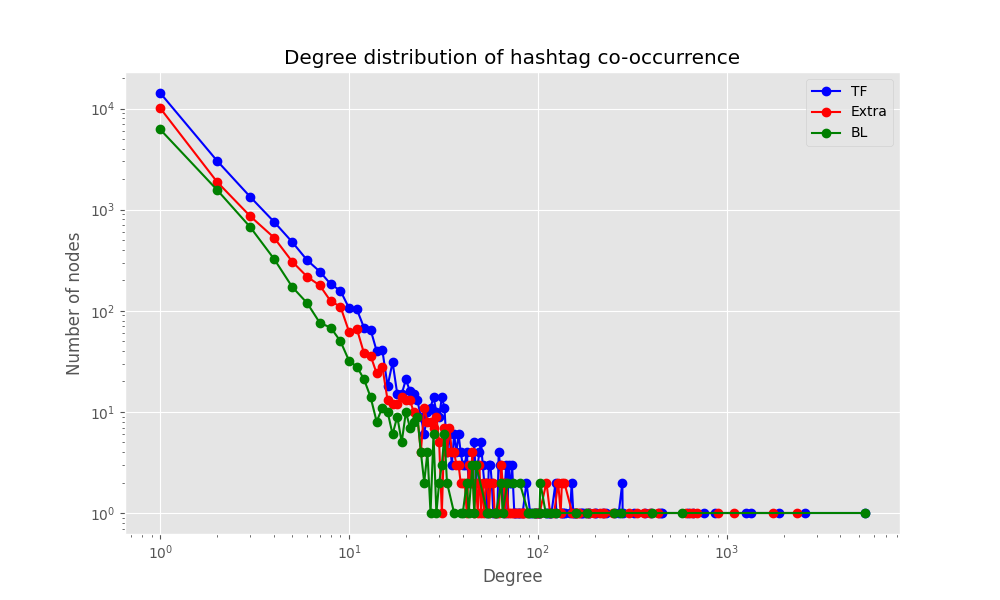
\includegraphics[width=\linewidth]{./images/degree_distribution.png}}
		\caption{Degree distribution of nodes for each dataset on a log-log graph.}
		\label{degree_distribution}
	\end{figure}
	
	\subsection{Basic Network Statistics}
		\begin{tabularx}{0.95\linewidth}{| l | X | X | X |}
			\hline
			 \, & \textbf{BL} & \textbf{AD} & \textbf{EX} \\ \hline
			 \textbf{Number of Nodes} & 10,777 & 24,653 & 16,787 \\ \hline
			 \textbf{Number of Edges} & 24,549 & 86,857 & 64,055 \\ \hline
			 \textbf{Network Diameter} & 8 & 9 & 9 \\ \hline
			 \textbf{Avg. Path Length} & 2.61 & 3.090 & 3.292 \\ \hline
			 \textbf{Average Degree} & 4.556 & 7.047 & 7.632 \\ \hline
			 \textbf{Avg. Clustering Coefficient} & 0.858 & 0.864 & 0.871 \\ \hline
			 \textbf{Modularity} & 0.374 & 0.607 & 0.565 \\ \hline
			 \textbf{Eigenvector Centrality} & 0.257 & 0.349 & 0.291 \\ \hline
		\end{tabularx}

\section{Approach}
	\subsection{Louvain Community Detection}
		{
			We chose to use the Louvain agglomerative community detection algorithm \cite{louvain} because it runs quickly whilst also maximising the modularity at every step. It is also the algorithm implemented by Gephi to calculate the modularity of a graph so we should see similar partitions to those produced by Gephi and should find a similar, if not exactly the same, number of communities. \\
			
			The community detection algorithm is implemented using the Python igraph \cite{igraph} implementation. First a weighted edge list is produced from the datasets where each vertex represents a hashtag, an edge represents that the hashtags co-occur, and the edge weight represents the frequency with which they have co-occurred. From this we create a graph using igraph and call its \texttt{community\_multilevel} method to perform the community detection which returns a \texttt{VertexClustering} object which can be iterated over; at each iteration a community division of co-occurring hashtags is returned. We need to save the resulting community divisions to perform sentiment analysis later, so we use this to create a dictionary where the key is the community index and the value is the community division. Finally we save the dictionary as a JSON file which can easily be loaded later.
		\par}
	
	\subsection{Sentiment Analysis: Naïve Bayes Classifier}
		{
			The use of natural language processing is required in order to identify the overall ‘sentiment’ of an identified community of tweets from the given dataset. Sentiment refers to the overall view or opinion that is expressed in the tweets of each community. In our case, we have chosen to build a naïve Bayes classifier to do this which works by classifying the communities on overall positive, negative or neutral sentiment. \\
			
The classifier is implemented as follows. It loads in a train and test data set. The test dataset is the set of tweets for a given community and the train data set is a precompiled set of words/phrases that are labelled (‘positive’, ‘negative’ or ‘neutral’). The training data set is used to train the classifier based on training features that are extracted from the train data set. Once the classifier has been trained, it can then be used to identify the overall sentiment of the unseen given test data set, which in our case is the set of tweets for a particular community. The classifier goes through the community tweets and applies a label to each based on what it thinks the sentiment of it is. When this has been completed, the labels are summed and the label with the highest count is considered the overall sentiment of the community.
		\par}
		
	\subsection{EXTENSION}		
		\subsubsection{Task 1: Path Length and Clustering Coefficients}
			{
				This section of the extension work looks at the difference between the path lengths and clustering coefficients of the Adaptive network in comparison to the average of three generated random graphs with the same number of nodes and a similar number of edges. \\
 
				The random graphs were generated using the Erdos-Renyi model in which each edge of a given node has a fixed probability of being absent or present, independently of the other edges. To achieve a number of edges close to that of the Adaptive network, the probability of each random network was set to 0.000029. This produced the given graphs: \\
				
			\begin{tabularx}{0.95\linewidth}{| p{0.2\linewidth} | X | X |}
				\hline
				\textbf{Random Network} & \textbf{Number of Nodes} & \textbf{Number of Edges} \\ \hline
				1 & $24,653$ & $91,125$ \\ \hline
				2 & $24,653$ & $91,138$ \\ \hline
				3 & $24,653$ & $90,676$ \\ \hline
			\end{tabularx}
			\\ \\ \\
			The NetworkX Python library \cite{networkx} was utilised for the creation of the three random graphs and the computation of the clustering coefficients and path lengths. The \texttt{gnp\_random\_graph(n,p)} method was used to generate the three random graphs, and in order to read the Adaptive network into NetworkX, it was converted from a Gephi network to Graphml which is compatible with NetworkX.
			\par}
			
		\subsubsection{Task 2: Which is more robust?}
			{
				Network robustness can be defined as the ability of a network to continue performing well when it is subject to failures or attacks \cite{robustness}. In this section, the network robustness of the AD dataset will be assessed in comparison to the robustness of three random networks constructed in the G(n,p) Erdős–Rényi model. \\

				In order to assess the robustness of the networks, a targeted attack was performed by removing nodes based on node degree. The top 0.01\%, 0.1\%, 1\% and 10\% highest degree nodes were removed and the effect of this on the giant component of the networks was recorded. After removing the nodes each time, the number of nodes, edges, average path length and average node degree was recorded of the new giant component. \\

				The method involved importing the datasets into Gephi, deleting the top \% highest degree nodes using the data laboratory feature. The giant component was then shown using the filtering tool and the relevant statistics were computed.
			\par}
		
		
		\subsubsection{Task 3: PageRank}	
			{
				This task will examine the computed average page rank values for the original AD dataset and the three randomly generated networks. \\
				
				The PageRank values were calculated using Gephi. The probability p, which is used to simulate the user randomly restarting the web surfing, was set to 0.85, and the stopping criterion value was set to 0.001.
			\par}
			
			
		\subsubsection{Task 4: Cascade}
			
			

\section{Results}
	\subsection{Community Detection}
	
	\subsection{Sentiment Analysis}
	
	\subsection{EXTENSION}
		\subsubsection{Task 1: Clustering Coefficient}
			{
				The average clustering coefficient was then computed for each network by dividing the sum of all clustering coefficients by the number of nodes available. The results of the Adaptive network and the average of the three random networks are provided in the table below. \\
				
				\begin{tabularx}{0.95\linewidth}{| X | X |}
					\hline
					\, & \textbf{Average Clustering Coefficient} \\ \hline
					\textbf{AD Network} & $0.6109340628572504$ \\ \hline
					\textbf{Random Network Average} & $0.0002252434124308$ \\ \hline
				\end{tabularx} 
				\\ \\ \\
				It is evident that the average clustering coefficient over all of the nodes in the Adaptive network are significantly higher than the average of the three random networks, which suggests that the neighbouring nodes in the Adaptive network are more densely connected.  Evidence suggests that nodes tend to establish more tightly knit groups in real-world networks, such as the Adaptive network, in comparison to random networks which establish links between two nodes at random \cite{hollandleinhardt}.
			\par}
			
			\begin{figure}[htbp]
				\centerline{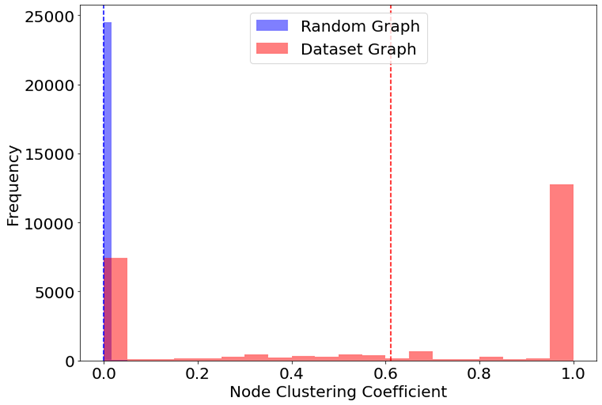
\includegraphics[width=\linewidth]{./images/random_ad_clustering.png}}
				\caption{The distributions of clustering coefficients compared between a random graph and AD graph.}
				\label{random_clustering}
			\end{figure}
			
			{
				As illustrated in the figure above, the clustering coefficient of each node in the Adaptive graph is frequently high which further implies that the real-world social network has tightly knit groups in comparison to those of the random graphs which consists of nodes most frequently distributed in the low clustering coefficients.
			\par}
		
		\subsubsection{Task 1: Path Length}
			{
				The same process was utilised as discussed in the clustering coefficient section to generate the three random networks and read in the Adaptive network into NetworkX to compute the average path length. \\
				
				To obtain the averages, the NetworkX \texttt{shortest\_path} function was used to compute the shortest paths between each source and target node in a given network which were then stored in a list. The sum of the shortest paths were then divided by the total number of entries in the list, which provided the average path length. This process was used for the Adaptive network and the three random networks. \\

				\begin{tabularx}{0.95\linewidth}{| X | X |}
					\hline
					\, & \textbf{Average Path Length} \\ \hline
					\textbf{AD Network} & $3.090$ \\ \hline
					\textbf{Random Network Average} & $5.288$ \\ \hline
				\end{tabularx}
				\\ \\ \\
				The average number of steps along the shortest path for all possible pairs of the network nodes were significantly less in the Adaptive network. This further ties in with the evidence provided for real-world networks having a higher clustering coefficient when compared to random networks as a tightly knitted network also implies that traversal through the network to get from a given source to destination node will be shorter.
			\par}
			
		\subsubsection{Task 2: Which is more robust? (AD Dataset)}
			{
				This section shows the results of removing nodes on the AD dataset. The impact of removing nodes on the average path length and average degree is represented with the following graph. \\ \\
				\begin{tabularx}{0.95\linewidth}{| X | X | X | X | X |}
					\hline
					\textbf{Nodes removed} & \textbf{Number of nodes} & \textbf{Number of edges} & \textbf{Path length} & \textbf{Average node degree} \\ \hline
					$0\%$ & $23,733$ & $86,355$ & $3.09$ & $7.277$ \\ \hline
					$0.01\%$ & $20,773$ & $76,809$ & $3.369$ & $7.395$ \\ \hline
					$0.1\%$ & $15,861$ & $55,248$ & $4.141$ & $6.967$ \\ \hline
					$1\%$ & $11,000$ & $28,444$ & $6.279$ & $5.172$ \\ \hline
					$10\%$ & $12,135$ & $18,861$ & $2.966$ & $3.109$ \\ \hline
				\end{tabularx}
			\par}
			\begin{figure}[htbp]
				\centerline{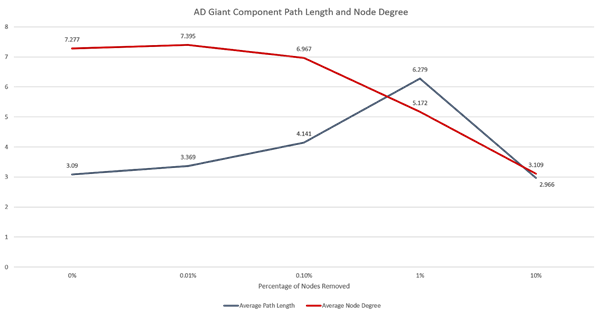
\includegraphics[width=\linewidth]{./images/robust_ad_path.png}}
				\label{robust_ad_path}
			\end{figure}
			{
				The graph shows that as nodes were removed from the network, the average node degree decreased of the resulting giant component each time. The graph also shows that as nodes were removed, the average path length increased up until 1\% of the highest degree nodes were removed. At 10\% node removal, the average path length decreased from 6.279 to 2.966. \\
				
				The impact of removing nodes on the number of nodes and edges (size) of the resulting giant component each time is shown by the following graph.
			\par}
			\begin{figure}[htbp]
				\centerline{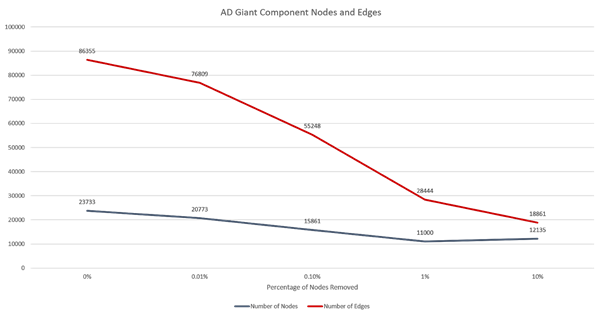
\includegraphics[width=\linewidth]{./images/robust_ad_component.png}}
				\label{robust_ad_component}
			\end{figure}
			{
				The graph shows that as nodes were removed, the number of edges of the resulting giant component decreased each time. Similarly, the number of nodes also decreases each time up until 1\%. However, at 10\% node removal, the number of nodes in the giant component increased from 11,000 to 12,135.
			\par}
			
		\subsubsection{Task 2: Which is more robust? (Random Graphs)}
			{
				This section shows the average results of removing nodes of the three generated random networks with comparable nodes/edges to the AD dataset. The impact of removing nodes on the average path length and node degree of the resulting giant component is shown below. \\ \\
				\begin{tabularx}{0.95\linewidth}{| X | X | X | X | X |}
					\hline
					\textbf{Nodes removed} & \textbf{Number of nodes} & \textbf{Number of edges} & \textbf{Path length} & \textbf{Average node degree} \\ \hline
					$0\%$ & $24,638$ & $91,125$ & $5.284$ & $7.397$ \\ \hline
					$0.01\%$ & $24,636$ & $91,086$ & $5.296$ & $7.395$ \\ \hline
					$0.1\%$ & $24,613$ & $90,683$ & $5.284$ & $7.369$ \\ \hline
					$1\%$ & $24,389$ & $87,324$ & $5.374$ & $7.161$ \\ \hline
					$10\%$ & $22,132$ & $62,981$ & $6.038$ & $5.691$ \\ \hline
				\end{tabularx}
			\par}
			\begin{figure}[htbp]
				\centerline{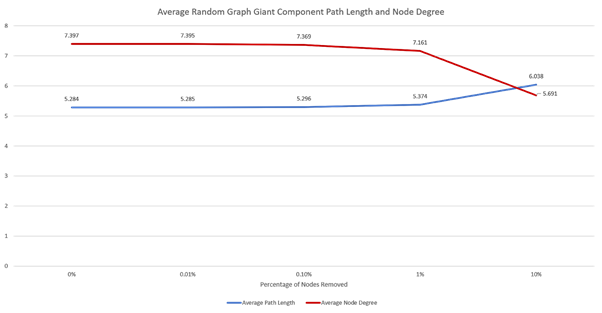
\includegraphics[width=\linewidth]{./images/robust_random_path.png}}
				\label{robust_random_path}
			\end{figure}
			{
				The graph shows that average path length increases slightly as nodes are removed, with the largest increase from 1\% to 10\% node removal. Similarly, the average node degree decreases slightly with the largest decrease from 1\% to 10\% node removal. The impact on the size of the giant component for the random graphs is shown in the following graph.
			\par}
			\begin{figure}[htbp]
				\centerline{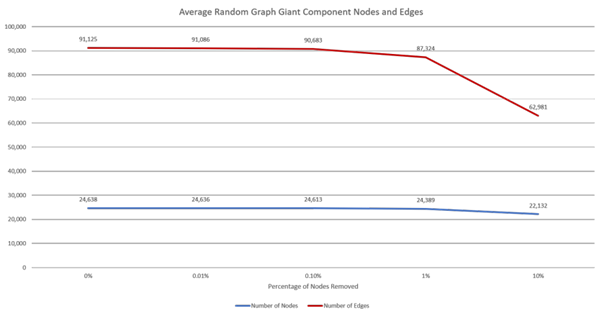
\includegraphics[width=\linewidth]{./images/robust_random_component.png}}
				\label{robust_random_component}
			\end{figure}
			{
				The graph shows that the number of nodes and edges both decreases as nodes were removed. The largest decrease occurred in the number of edges from 1\% to 10\% node removal.
			\par}
		
		\subsubsection{Task 3: PageRank (AD Dataset)}
			{
				The following graph represents the distribution of page rank values for each node in the original AD dataset.
			\par}
			\begin{figure}[htbp]
				\centerline{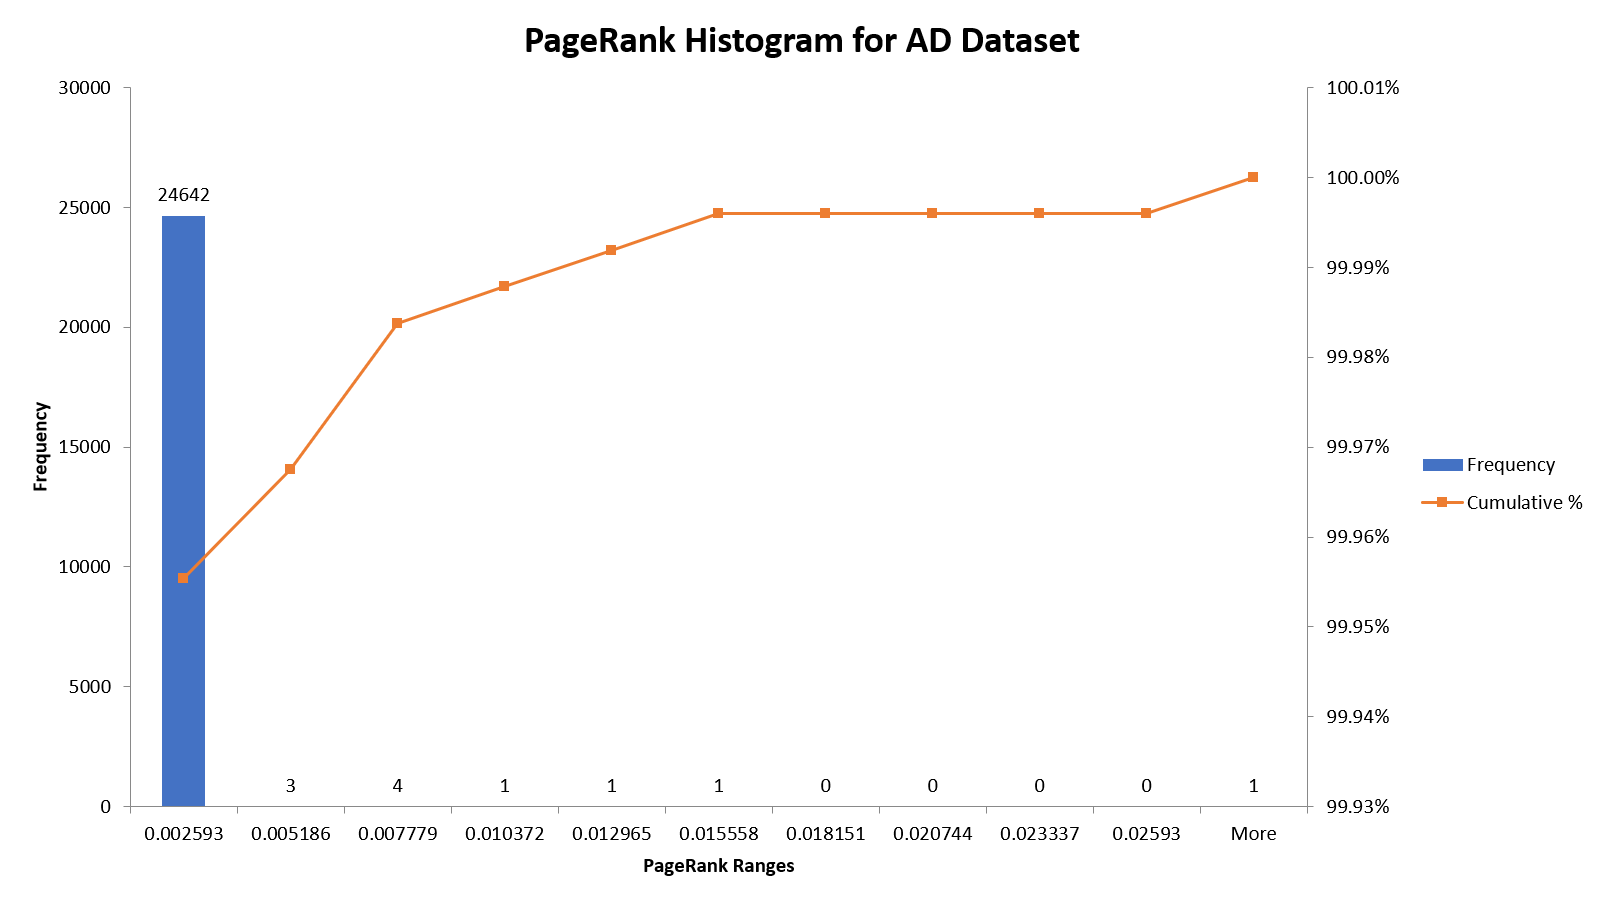
\includegraphics[width=\linewidth]{./images/pagerank_ad.png}}
				\label{pagerank_ad}
			\end{figure}
			{
				The graph shows that the page rank values for this dataset were heavily positively skewed. This is due to the fact that the majority of the nodes scored very low with a value of 0 after the page rank algorithm was conducted. $99.96\%$ of the nodes fell within the range $[0, 0.0002593]$. This is because most of these hashtags were random and not very common in the dataset compared to a hashtag such as \texttt{glastonbury}. Only $11$ nodes fell within ranges higher than this. The highest ranking node was the node corresponding to the hashtag \texttt{glastonbury} at a value of $0.039718$. This is because a large portion of the people at the Glastonbury event were tweeting with this hashtag, hence this node receiving many more links than other nodes, resulting in having more importance.\\
				
				The original AD dataset had an average page rank value $0.0000402863748833827$.
			\par}
			
		\subsubsection{Task 3: PageRank (Random Graphs)}
			{
				The PageRank algorithm was applied to the three randomly generated networks. The following histograms show the distribution of the page rank scores of the nodes in the network.
			\par}
			\begin{figure}[htbp]
				\centerline{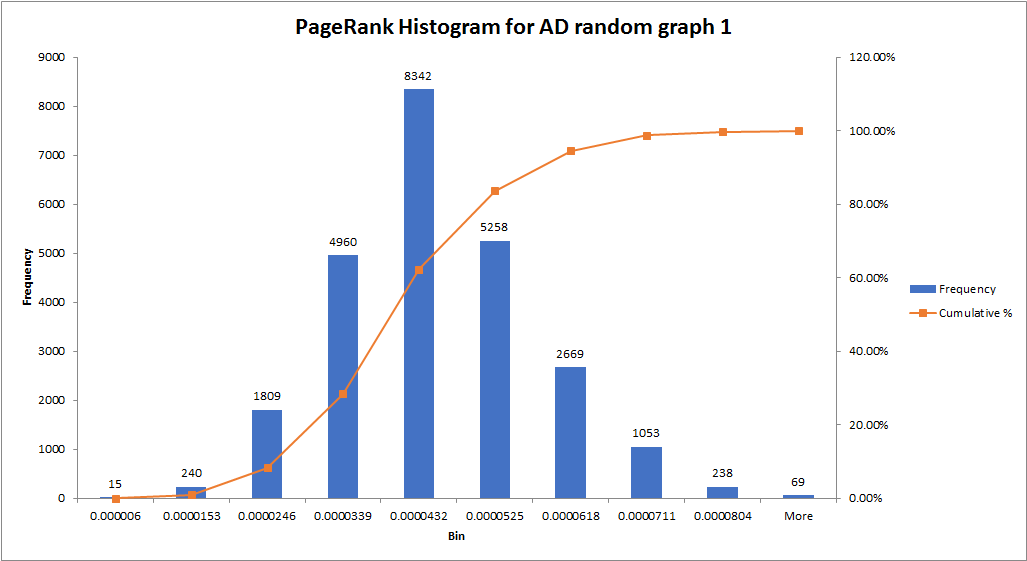
\includegraphics[width=\linewidth]{./images/pagerank_random1.png}}
				\label{pagerank_random1}
			\end{figure}
			\begin{figure}[htbp]
				\centerline{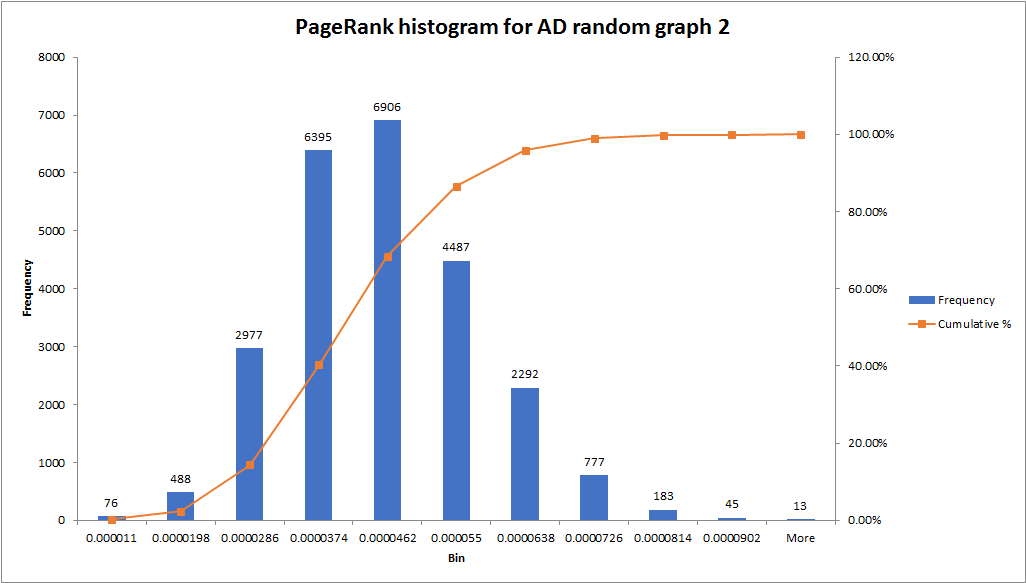
\includegraphics[width=\linewidth]{./images/pagerank_random2.png}}
				\label{pagerank_random2}
			\end{figure}
			\begin{figure}[htbp]
				\centerline{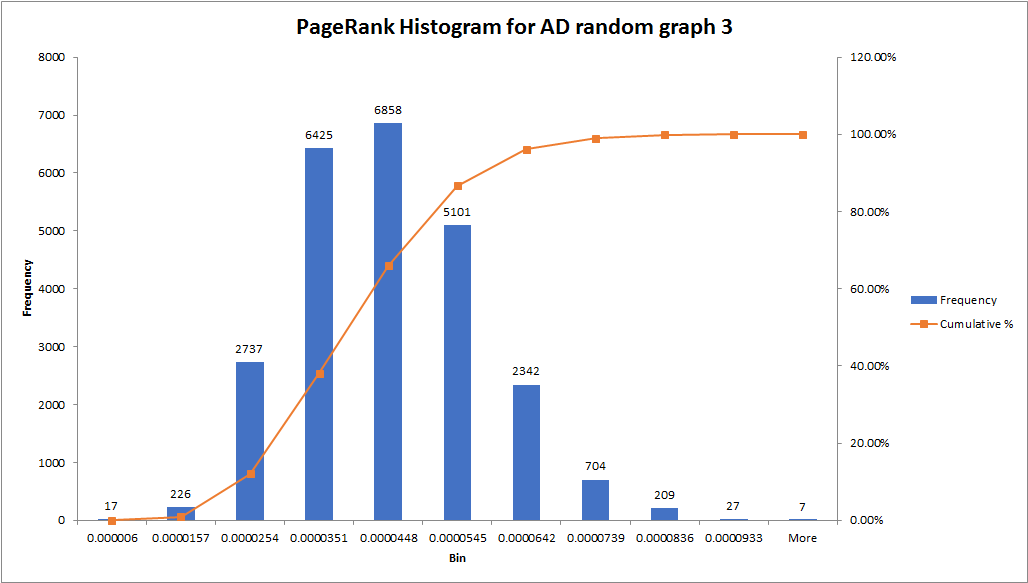
\includegraphics[width=\linewidth]{./images/pagerank_random3.png}}
				\label{pagerank_random3}
			\end{figure}
			{
				As seen in the graphs, the distributions are much more uniform than the original AD dataset. The average page rank scores of the generated graphs are shown in the following table. \\ \\
				\begin{tabularx}{0.95\linewidth}{| X | X |}
					\hline
					\textbf{Random Graph} & \textbf{Average Page Rank} \\ \hline
					$1$ & $0.0000405641098446437$ \\ \hline
					$2$ & $0.0000405856568854253$ \\ \hline
					$3$ & $0.0000405617977528091$ \\ \hline
				\end{tabularx}
			\par}
			
		\subsubsection{Task 4: Cascade}	
			
			
			
\section{Conclusions}
	\subsection{EXTENSION}
		\subsubsection{Task 2: Which is more robust?}
			{
				The robustness of a network can be assessed by its level of connectivity. The quantitative measures used in this project to assess the robustness of the networks are average path length. These measures are being used under the fact that the shorter the path length, the more robust the network is \cite{robustness}. \\
				
The average path length of the random graphs increased from 5.284 to 5.374 resulting in a 1.7\% increase. Looking at the original AD dataset, the path length increased from 3.09 to 6.279 equating to a 103.2\% increase. In this period, the random graph is much more robust. However, considering the change from 1\% to 10\%, the AD dataset actually decreased by 52.7\%. \\

Overall, the AD dataset actually became more robust after 10\% node removal whereas the random graph became less robust with 10\% node removal. However, the rate at which the random graph became less robust was significantly lower than the AD dataset. Across all values computed, The AD dataset’s giant component statistics increased more each time meaning it responded more erratically than the random graphs. 
			\par}
		
		\subsubsection{Task 3: PageRank}
			{
				The page rank values for the AD dataset averaged out to a value of $0.0000402863748833827$. This value is comparable to the random graphs shown in the above table. 
			\par}
			
		\subsubsection{Task 4: Cascade}

\section*{References}

Please number citations consecutively within brackets \cite{gnewman}. The 
%sentence punctuation follows the bracket \cite{b2}. Refer simply to the reference 
%number, as in \cite{b3}---do not use ``Ref. \cite{b3}'' or ``reference \cite{b3}'' except at 
%the beginning of a sentence: ``Reference \cite{b3} was the first $\ldots$''

Number footnotes separately in superscripts. Place the actual footnote at 
the bottom of the column in which it was cited. Do not put footnotes in the 
abstract or reference list. Use letters for table footnotes.

Unless there are six authors or more give all authors' names; do not use 
``et al.''. Papers that have not been published, even if they have been 
%submitted for publication, should be cited as ``unpublished'' \cite{b4}. Papers 
%that have been accepted for publication should be cited as ``in press'' \cite{b5}. 
Capitalize only the first word in a paper title, except for proper nouns and 
element symbols.

For papers published in translation journals, please give the English 
%citation first, followed by the original foreign-language citation \cite{b6}.

\begin{thebibliography}{00}
	\bibitem{gnewman} M. Girvan, and M. E. J. Newman. "Community structure in social and biological networks". Proceedings of the National Academy of Sciences, Jun 2002, 99 (12), pp. 7821-7826
	\bibitem{cnewman} A. Clauset, M. E. J. Newman, and C. Moore. "Finding community structure in very large networks". Physical Review E, Dec 2004, 70 (6)
	\bibitem{louvain} V. D. Blondel, J. Guillaume, R. Lambiotte, and E. Lefebvre. "Fast unfolding of communities in large networks". Journal of Statistical Mechanics: Theory and Experiment, Oct 2008, 2008 (10)
	\bibitem{strim} L. Tokarchuk, X. Wang, S. Poslad. "Piecing together the puzzle: Improving event content coverage for real-time sub-event detection using adaptive microblog crawling". PLoS ONE 12 (11)
	\bibitem{igraph} G. Csardi, and T. Nepusz. "The igraph software package for complex network research". InterJournal, 2006, Complex Systems, pp. 1695
	\bibitem{networkx} A. Hagberg, D. Schult, and P. Swart, “Exploring network structure, dynamics, and function using NetworkX”, in Proceedings of the 7th Python in Science Conference (SciPy2008), Gäel Varoquaux, Travis Vaught, and Jarrod Millman (Eds), (Pasadena, CA USA), pp. 11–15, Aug 2008
	\bibitem{hollandleinhardt} P. Holland, and S. Leinhardt. "Transitivity in Structural Models of Small Groups". Comparative Group Studies, 1971, 2(2), pp. 107–124.
	\bibitem{robustness} W. Ellens, and R. Kooji. "Graph measures and network robustness".  arXiv:1311.5064, Nov 2013
	%\bibitem{b1} G. Eason, B. Noble, and I. N. Sneddon, ``On certain integrals of Lipschitz-Hankel type involving products of Bessel functions,'' Phil. Trans. Roy. Soc. London, vol. A247, pp. 529--551, April 1955.
	%\bibitem{b2} J. Clerk Maxwell, A Treatise on Electricity and Magnetism, 3rd ed., vol. 2. Oxford: Clarendon, 1892, pp.68--73.
	%\bibitem{b3} I. S. Jacobs and C. P. Bean, ``Fine particles, thin films and exchange anisotropy,'' in Magnetism, vol. III, G. T. Rado and H. Suhl, Eds. New York: Academic, 1963, pp. 271--350.
	%\bibitem{b4} K. Elissa, ``Title of paper if known,'' unpublished.
	%\bibitem{b5} R. Nicole, ``Title of paper with only first word capitalized,'' J. Name Stand. Abbrev., in press.
	%\bibitem{b6} Y. Yorozu, M. Hirano, K. Oka, and Y. Tagawa, ``Electron spectroscopy studies on magneto-optical media and plastic substrate interface,'' IEEE Transl. J. Magn. Japan, vol. 2, pp. 740--741, August 1987 [Digests 9th Annual Conf. Magnetics Japan, p. 301, 1982].
	%\bibitem{b7} M. Young, The Technical Writer's Handbook. Mill Valley, CA: University Science, 1989.
\end{thebibliography}


\section{Styling figs and stuff}
\subsection{Figures and Tables}
\paragraph{Positioning Figures and Tables} Place figures and tables at the top and 
bottom of columns. Avoid placing them in the middle of columns. Large 
figures and tables may span across both columns. Figure captions should be 
below the figures; table heads should appear above the tables. Insert 
figures and tables after they are cited in the text. Use the abbreviation 
``Fig.~\ref{fig}'', even at the beginning of a sentence.

\begin{table}[htbp]
\caption{Table Type Styles}
\begin{center}
\begin{tabular}{|c|c|c|c|}
\hline
\textbf{Table}&\multicolumn{3}{|c|}{\textbf{Table Column Head}} \\
\cline{2-4} 
\textbf{Head} & \textbf{\textit{Table column subhead}}& \textbf{\textit{Subhead}}& \textbf{\textit{Subhead}} \\
\hline
copy& More table copy$^{\mathrm{a}}$& &  \\
\hline
\multicolumn{4}{l}{$^{\mathrm{a}}$Sample of a Table footnote.}
\end{tabular}
\label{tab1}
\end{center}
\end{table}

\begin{figure}[htbp]
%\centerline{\includegraphics{fig1.png}}
\caption{Example of a figure caption.}
\label{fig}
\end{figure}

Figure Labels: Use 8 point Times New Roman for Figure labels. Use words 
rather than symbols or abbreviations when writing Figure axis labels to 
avoid confusing the reader. As an example, write the quantity 
``Magnetization'', or ``Magnetization, M'', not just ``M''. If including 
units in the label, present them within parentheses. Do not label axes only 
with units. In the example, write ``Magnetization (A/m)'' or ``Magnetization 
\{A[m(1)]\}'', not just ``A/m''. Do not label axes with a ratio of 
quantities and units. For example, write ``Temperature (K)'', not 
``Temperature/K''.

\section*{Acknowledgment}

The preferred spelling of the word ``acknowledgment'' in America is without 
an ``e'' after the ``g''. Avoid the stilted expression ``one of us (R. B. 
G.) thanks $\ldots$''. Instead, try ``R. B. G. thanks$\ldots$''. Put sponsor 
acknowledgments in the unnumbered footnote on the first page.

\end{document}
